\section{Die graphische Oberfläche}
Aus den minimalen Anforderungen an die graphische Oberfläche ergibt sich das Design.
Anhand der folgenden Abbildungen werden die gefertigten Entwürfe der BenutzerInnenoberfläche dargestellt.\\\\
Diese Listenansicht in Abbildung \ref{fig:list} besteht aus dem Header / Kopf und den Listeneinträgen.
Sie zeigt die Kontakteinträge in beiden Netzwerkstatus: online (Abbildung \ref{fig:list-online}) und offline (\ref{fig:list-offline}).\\\\
%
%
Im Header ist abzulesen, ob die Anwendung gerade eine Netzwerkverbindung hat oder nicht.
Für eine bessere Prägnanz wurden hierzu unterstützend die Farben Rot für keine Verbindung und Grün für eine bestehende Netzwerkverbindung gewählt.
Rechts im Header gibt es einen Knopf, mit dem man in die Ansicht gelangt, in der ein Kontakt hinzugefügt werden kann.\\
%
In der Liste sieht man die Namen der Person und jeweils einen Knopf zum Bearbeiten oder Löschen.
Mit der Betätigung des `Delete`--Knopfs wird der entsprechende Eintrag in der Liste gelöscht
\begin{figure}[H]
  \centering
  \begin{subfigure}[t]{0.49\textwidth}
          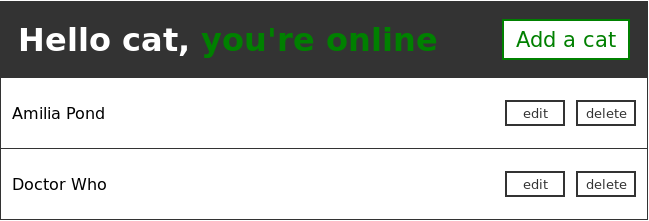
\includegraphics[width=\textwidth]{list-online}
          \caption{Kontaktliste im Onlinestatus}
          \label{fig:list-online}
  \end{subfigure}
  ~ 
  \begin{subfigure}[t]{0.49\textwidth}
          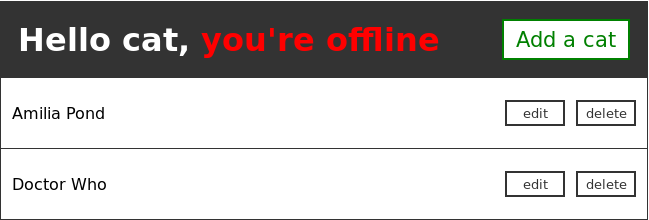
\includegraphics[width=\textwidth]{list-offline}
          \caption{Kontaktliste im Offlinestatus}
          \label{fig:list-offline}
  \end{subfigure}
  \grayRule
  \caption{Die Kontaktliste in beiden Netzwerkstatus}
  \label{fig:list}
\end{figure}
Klickt man auf den Knopf zum Bearbeiten oder auf den zum Hinzufügen eines Kontakts, gelangt man in die Bearbeitungsansicht (vgl. Abbildung \ref{fig:edit}). Der Header ist bis auf den Knopf zum Hinzufügen eines Kontakts identisch zu dem der Liste. Auch hier ist abzulesen, ob die Anwendung on-- oder offline ist. Da man sich bereits in der Ansicht zum Anlegen oder Editieren eines Kontaks befindet, ist der Knopf im Header überflüssig.\\
Ein Kontakt hat einen Namen, eine E-Mailadresse und eine Telefonnummer. In dieser Ansicht gibt es für jedes Attribut ein Eingabefeld. Die Felder sind beim Bearbeiten des Kontakts vorausgefüllt. Mittels Betätigung des ''Speichern'' Knopfs werden die Änderungen übernommen, klickt man auf ''Cancel'', werden sie verworfen. In beiden Fällen gelangt man wieder zur Listenansicht.
\begin{figure}[H]
  \centering
  \begin{subfigure}[t]{0.49\textwidth}
          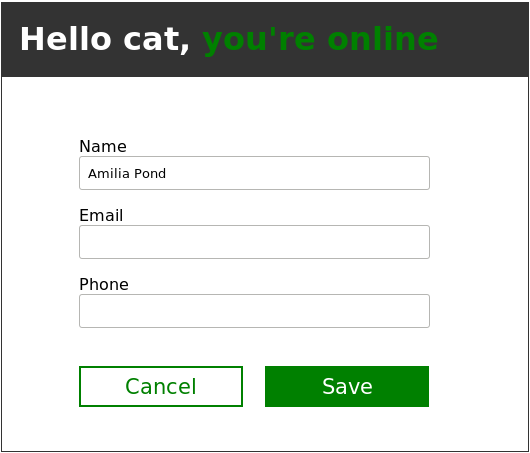
\includegraphics[width=\textwidth]{edit}
          \caption{Editieransicht im Onlinestatus}
          \label{fig:edit-online}
  \end{subfigure}
  ~ 
  \begin{subfigure}[t]{0.49\textwidth}
          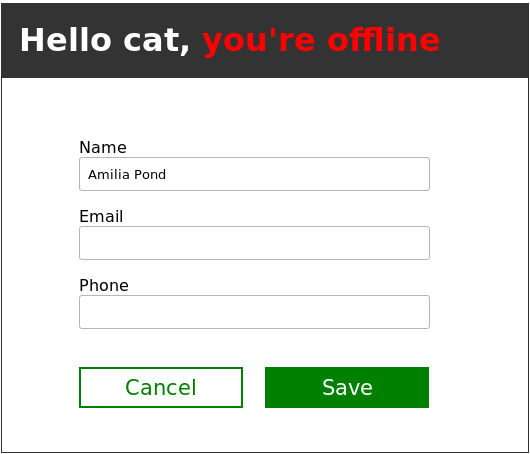
\includegraphics[width=\textwidth]{edit-offline}
          \caption{Editieransicht im Offlinestatus}
          \label{fig:edit-offline}
  \end{subfigure}
  \grayRule
  \caption{Die Editieransicht in beiden Netzwerkstatus}
  \label{fig:edit}
\end{figure}
Sobald ein Konflikt entstanden ist, soll sich ein Dialog öffnen, der die nutzenden Personen darüber informiert, welcher Kontakteintrag konfliktbehaftet ist und mit welcher Version er konkurriert.
Anhand des Dialoginhalts kann unterschieden werden, welche Version die lokal gespeicherte ist und welche vom Server kommt.
Der Dialog beinhaltet außerdem zwei unterschiedlich farbige Knöpfe, die jeweils den Kontakteintrag in einer anderen Version anzeigen.
Durch Klick auf einen Knopf wird die bevorzugte Version des Kontakts gespeichert und die andere verworfen.
So kann ein Mensch entscheiden, welche Version behalten werden soll und es wird sichergestellt, dass keine Daten verloren gehen.\\
Für die Implementierung des Konfliktdialogs ist es notwendig, dass die zu untersuchenden Technologien die Möglichkeit bieten, Konflikte zu speichern oder wenigstens als solche zu identifizieren, sodass sie manuell gespeichert werden können.